% !TEX program = xelatex
\documentclass[UTF8,fontset=fandol,a4paper,11pt]{ctexart}
\usepackage[margin=21mm,top=23mm,bottom=22mm,headheight=16pt]{geometry}
\usepackage{amsmath,amssymb,mathtools,bm}
\usepackage{tikz}
\usetikzlibrary{arrows.meta,calc,angles,quotes,patterns,decorations.pathmorphing}
\usepackage{xcolor,booktabs,array,longtable,enumitem,fancyhdr,needspace}
\usepackage[unicode,hidelinks]{hyperref}
\definecolor{ink}{HTML}{24343C}
\definecolor{accent}{HTML}{166A70}
\definecolor{muted}{HTML}{65747A}
\definecolor{rulegray}{HTML}{D4DDE0}
\definecolor{warm}{HTML}{966037}
\color{ink}
\setlength{\parindent}{2em}
\setlength{\parskip}{4pt}
\linespread{1.12}
\AtBeginDocument{\setlength{\abovedisplayskip}{6pt plus 2pt minus 1pt}
\setlength{\belowdisplayskip}{6pt plus 2pt minus 1pt}
\setlength{\abovedisplayshortskip}{0pt plus 1pt}
\setlength{\belowdisplayshortskip}{4pt plus 1pt}}
\setlist[enumerate]{label=(\arabic*),leftmargin=2.3em,itemsep=3pt,topsep=4pt}
\setlist[itemize]{leftmargin=2em,itemsep=2pt,topsep=4pt}
\allowdisplaybreaks[1]
\setlength{\emergencystretch}{2em}
\setcounter{secnumdepth}{0}
\providecommand{\tightlist}{\setlength{\itemsep}{0pt}\setlength{\parskip}{0pt}}
\ctexset{section={format=\Large\bfseries\color{accent},beforeskip=10pt,afterskip=9pt},
subsection={format=\normalsize\bfseries\color{accent},beforeskip=10pt,afterskip=4pt},
subsubsection={format=\normalsize\bfseries,beforeskip=8pt,afterskip=3pt}}
\pagestyle{fancy}
\fancyhf{}
\fancyhead[L]{\small\color{muted}物理学难题集萃}
% 页眉仅保留书名；版本名称只在封面显示。
\fancyfoot[L]{\small\color{muted}\chapterlabel}
\fancyfoot[R]{\small\thepage}
\renewcommand{\headrulewidth}{0.4pt}
\renewcommand{\footrulewidth}{0pt}
\newcommand{\dd}{\mathop{}\!\mathrm{d}}
\newcommand{\vect}[1]{\bm{#1}}
\newcommand{\tagline}[1]{\noindent{\small\color{muted}#1}\par}
\newcommand{\result}[1]{\begin{equation*}\boxed{#1}\end{equation*}}
\newcommand{\figcaption}[1]{\par\vspace{2pt}{\small\color{muted}#1}\par}
\newcommand{\teach}[2]{\Needspace{4\baselineskip}\subsection*{讲解要点与追问}#1\par\smallskip\noindent\textbf{追问：}#2\par}
\newcommand{\workarea}{\par\vspace{7mm}\noindent{\small\color{muted}作答区}\par\vspace{4mm}
\noindent\textcolor{rulegray}{\rule{\linewidth}{0.3pt}}\par\vspace{16mm}
\noindent\textcolor{rulegray}{\rule{\linewidth}{0.3pt}}\par\vspace{16mm}
\noindent\textcolor{rulegray}{\rule{\linewidth}{0.3pt}}\par\vspace{16mm}
\noindent\textcolor{rulegray}{\rule{\linewidth}{0.3pt}}}
\tikzset{axis/.style={-{Stealth[length=2mm]},thin,color=muted},
motion/.style={-{Stealth[length=2.3mm]},thick,color=accent},
force/.style={-{Stealth[length=2.3mm]},thick,color=warm},
traj/.style={thick,color=accent},guide/.style={dashed,thin,color=muted},
object/.style={thick,color=ink},every node/.style={font=\small}}\widowpenalty=10000\clubpenalty=10000\displaywidowpenalty=10000

\newcommand{\chapterlabel}{第五章\quad 静力平衡}
\hypersetup{pdftitle={第五章 静力平衡·学生版},pdfauthor={},pdfsubject={第五章第1--12题}}
\begin{document}
\pdfbookmark[0]{第五章 静力平衡}{cover}
\thispagestyle{empty}
\vspace*{20mm}
\noindent{\Huge\bfseries 物理学难题集萃}\par\vspace{8mm}
\noindent{\LARGE 第五章\quad 静力平衡}\par\vspace{10mm}
\noindent{\Large\color{accent}学生版}\par\vspace{8mm}
\noindent\textcolor{accent}{\rule{\linewidth}{1pt}}\par\vspace{8mm}
\noindent 第 1--12 题\par\vspace{5mm}
\noindent 题目、题图与作答区。\par
\vfill\clearpage
\pdfbookmark[1]{题目目录}{contents}
\section*{题目目录}
\begin{longtable}{@{}>{\color{accent}\bfseries}r p{120mm}@{}}
\toprule 题号 & 题目\\\midrule
1 & 圆锥面上链环的张力 \\
2 & 水平杆靠墙的摩擦条件 \\
3 & 竖杆受水平力的防滑条件 \\
4 & 半球凹面内的均匀细杆 \\
5 & 三圆柱堆放的摩擦下限 \\
6 & 斜木板上三球的支承 \\
7 & 分段悬线的平衡与提升功 \\
8 & 浮子与插杆的稳定性 \\
9 & 五杆悬挂的平衡形状 \\
10 & 厚木板在圆柱上的稳定性 \\
11 & 菱形木条与圆盘的平衡 \\
12 & 细绳张力与悬链线 \\
\bottomrule\end{longtable}


\clearpage

\pdfbookmark[2]{第 1 题 圆锥面上链环的张力}{q1}

\section*{第 1 题\quad 圆锥面上链环的张力}

\tagline{M-05-01}

顶角为 $\alpha$ 的圆锥体竖直固定，顶点在上。质量为 $m$、质量分布均匀的链环水平套在圆锥面上，处于静止状态。忽略链环与圆锥面之间的摩擦，$0<\alpha<\pi$。求链环中的张力。

\begin{center}\begin{minipage}{\linewidth}\centering
\begin{tikzpicture}
\draw[object] (-2,0)--(0,4)--(2,0);\draw[guide] (0,0)--(0,4);\draw[object] (0,1.6) ellipse (1.2 and .32);\draw (0,3.3) arc(-90:-116.57:.7);\node at (-.45,3.15) {$\alpha/2$};\node[right] at (1.3,1.6) {$m$};\node[below] at (0,-.1) {链环水平};
\end{tikzpicture}
\figcaption{图 5.1\quad 水平链环套在圆锥外侧，锥面母线与竖直轴夹角为 $\alpha/2$。}
\end{minipage}\end{center}

\workarea

\clearpage

\pdfbookmark[2]{第 2 题 水平杆靠墙的摩擦条件}{q2}

\section*{第 2 题\quad 水平杆靠墙的摩擦条件}

\tagline{M-05-02}

均匀杆 $AB$ 长为 $l$，重量为 $w_0$。$A$ 端接触粗糙竖直墙，$B$ 端用不可伸长的轻绳悬于墙上的 $C$ 点。杆水平，绳与杆的夹角为 $\theta$，$0<\theta<\pi/2$。
\begin{enumerate}\item 杆与墙的静摩擦系数 $\mu$ 满足什么条件时可以平衡？\item 在距 $A$ 为 $d$ 的位置悬挂重量 $w=w_0/2$ 的重物，$0\le d\le l$。求所需静摩擦系数的最小值与 $d$ 的关系。\end{enumerate}

\begin{center}\begin{minipage}{\linewidth}\centering
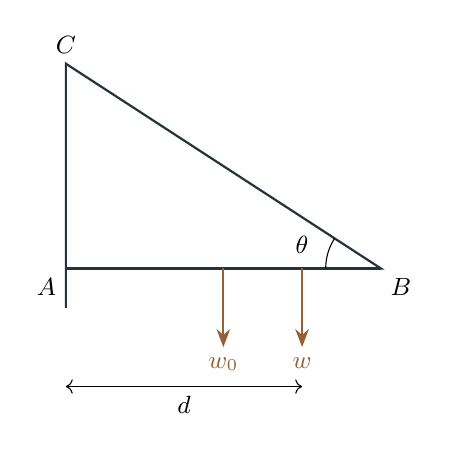
\begin{tikzpicture}
\coordinate(A)at(0,0);\coordinate(B)at(4,0);\coordinate(C)at(0,2.6);\draw[object] (0,-.5)--(C)--(B)--(A);\draw[object] (A)--(B);\draw (3.3,0) arc(180:147:.7);\node at (3.0,.3){$\theta$};\foreach \p/\pos in {A/below left,B/below right,C/above}{\node[\pos]at(\p){$\p$};}\draw[force] (2,0)--(2,-1)node[below]{$w_0$};\draw[force] (3,0)--(3,-1)node[below]{$w$};\draw[<->] (0,-1.5)--(3,-1.5)node[midway,below]{$d$};
\end{tikzpicture}
\figcaption{图 5.2\quad 杆端 $A$ 接触墙，$B$ 端用绳悬于 $C$，挂点距 $A$ 为 $d$。}
\end{minipage}\end{center}

\workarea

\clearpage

\pdfbookmark[2]{第 3 题 竖杆受水平力的防滑条件}{q3}

\section*{第 3 题\quad 竖杆受水平力的防滑条件}

\tagline{M-05-03}

质量为 $m$、长为 $L$ 的均匀细杆竖直放置，下端接触水平地面，静摩擦系数为 $\mu$。上端由轻绳拉住，绳的另一端固定在左下方，绳与竖杆的夹角为 $\theta$，$0<\theta<\pi/2$。在离地高度 $h$ 处向右施加水平力 $F$，$0\le h\le L$。求保持杆不滑倒所允许的 $F$ 的最大值，并讨论何时仅凭摩擦条件不能给出有限上限。

\begin{center}\begin{minipage}{\linewidth}\centering
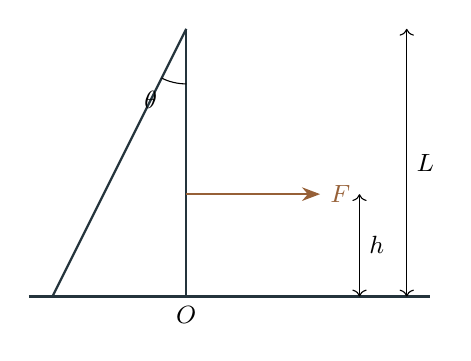
\begin{tikzpicture}
\draw[object](-2,0)--(3.1,0);
\draw[object](0,0)--(0,3.4);\draw[object](-1.7,0)--(0,3.4);
\draw(0,2.7)arc(-90:-116.565051177:.7);\node at(-.45,2.5){$\theta$};
\draw[force](0,1.3)--(1.7,1.3)node[right]{$F$};
\draw[<->](2.2,0)--(2.2,1.3)node[midway,right]{$h$};
\draw[<->](2.8,0)--(2.8,3.4)node[midway,right]{$L$};
\node[below]at(0,0){$O$};
\end{tikzpicture}
\figcaption{图5.3\quad 绳固定在左下方，推力高度$h$与杆长$L$分别标出。}\end{minipage}\end{center}

\workarea

\clearpage

\pdfbookmark[2]{第 4 题 半球凹面内的均匀细杆}{q4}

\section*{第 4 题\quad 半球凹面内的均匀细杆}

\tagline{M-05-04}

半径为 $R$ 的光滑半球形凹面内，一根刚性均匀细杆处于平衡。杆的一端接触内壁，杆身经过凹面边缘并伸出，如图所示。已知杆在凹面内的部分长为 $l$，求露出部分的长度，并给出该接触构型的适用范围。

\begin{center}\begin{minipage}{\linewidth}\centering
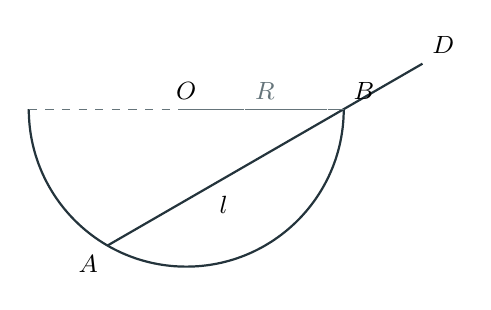
\begin{tikzpicture}
\coordinate(O)at(0,0);\coordinate(A)at(-1,-1.732050808);
\coordinate(B)at(2,0);\coordinate(D)at(3,.577350269);
\draw[object](-2,0)arc(180:360:2);\draw[guide](-2,0)--(2,0);
\draw[object](A)--(D);\draw[guide](O)--(B)node[midway,above]{$R$};
\node[above]at(O){$O$};\node[below left]at(A){$A$};
\node[above right]at(B){$B$};\node[above right]at(D){$D$};
\node[below right]at(.3,-.98){$l$};
\end{tikzpicture}
\figcaption{图5.4\quad 杆内端$A$接触凹面，杆身在边缘$B$处支承并伸出至$D$。}\end{minipage}\end{center}

\workarea

\clearpage

\pdfbookmark[2]{第 5 题 三圆柱堆放的摩擦下限}{q5}

\section*{第 5 题\quad 三圆柱堆放的摩擦下限}

\tagline{M-05-05}

三个半径和质量均相同的圆柱体互相接触，在水平地面上堆成两下、上一的对称构型。圆柱之间的静摩擦系数为 $\mu_1$，圆柱与地面之间为 $\mu_2$。求使三个圆柱静止所需的 $\mu_1$ 和 $\mu_2$ 的下限。

\begin{center}\begin{minipage}{\linewidth}\centering
\begin{tikzpicture}
\draw[object] (-2.4,0)--(2.4,0);\foreach \x/\y/\s in {-1/1/B,1/1/C,0/2.732/A}{\draw[object] (\x,\y)circle(1);\fill(\x,\y)circle(1.5pt);\node at(\x,\y+.25){$\s$};}\draw[guide] (-1,1)--(1,1)--(0,2.732)--cycle;\node[right]at(2,1.7){$r,m$ 相同};
\end{tikzpicture}
\figcaption{图 5.5\quad 三圆柱两两相切，圆心围成等边三角形。}
\end{minipage}\end{center}

\workarea

\clearpage

\pdfbookmark[2]{第 6 题 斜木板上三球的支承}{q6}

\section*{第 6 题\quad 斜木板上三球的支承}

\tagline{M-05-06}

均匀木板 $AB$ 长 $L=100\,\mathrm{cm}$，重 $2G$。$A$ 端铰接在竖直墙上，$B$ 端由水平轻绳拉住，木板与墙的夹角为 $60^\circ$。三个相同小球沿木板排列，彼此接触且都接触木板；最左球还接触墙。每球半径 $R=10\,\mathrm{cm}$，重 $G$。球与墙、木板以及球之间均光滑。求水平绳的张力 $T$。

\begin{center}\begin{minipage}{\linewidth}\centering
\begin{tikzpicture}
\coordinate(A)at(0,0);\coordinate(B)at(5.196152423,3);
\coordinate(E)at(.9,.519615242);\coordinate(F)at(1.939230485,1.119615242);
\coordinate(K)at(2.978460969,1.719615242);\coordinate(D)at(1.679422863,.969615242);
\draw[object](0,-.3)--(0,3.5);\draw[object](A)--(B)--(0,3);
\foreach \x/\y in {.6/1.039230485,1.639230485/1.639230485,2.678460969/2.239230485}
{\draw[object](\x,\y)circle(.6);}
\draw(0,.7)arc(90:30:.7);\node at(.45,.78){$60^\circ$};
\node[below]at(A){$A$};\node[right]at(B){$B$};
\node[above]at(3.7,3){水平绳};\node[below right]at(3.7,1.9){$L=10R$};
\end{tikzpicture}
\figcaption{图5.6\quad 三球与板、墙接触；木板长度及球半径按$L:R=10:1$绘制。}
\end{minipage}\end{center}

\workarea

\clearpage

\pdfbookmark[2]{第 7 题 分段悬线的平衡与提升功}{q7}

\section*{第 7 题\quad 分段悬线的平衡与提升功}

\tagline{M-05-07}

四段质量可忽略的细线 $AB,BC,CD,DE$ 长度均为 $5\,\mathrm m$，$A,E$ 固定于同一水平天花板，$AE=14\,\mathrm m$。$B,D$ 各挂质量 $m_0=7\,\mathrm{kg}$ 的小球，$C$ 挂质量 $m$ 的重物。平衡构型关于 $C$ 的竖直线对称，$C$ 距天花板 $7\,\mathrm m$。
\begin{enumerate}\item 求 $m$。\item 用外力缓慢提升 $C$，直到 $B,C,D$ 在同一水平线上，求外力做的功。取 $g=9.8\,\mathrm{m/s^2}$。\end{enumerate}

\begin{center}\begin{minipage}{\linewidth}\centering
\begin{tikzpicture}
\draw[object] (-3.5,0)--(3.5,0);\draw[object] (-3.5,0)--(-2,-2)--(0,-3.5)--(2,-2)--(3.5,0);\foreach \x/\y/\s in {-3.5/0/A,3.5/0/E,-2/-2/B,2/-2/D,0/-3.5/C}{\fill(\x,\y)circle(2pt);\node[above right]at(\x,\y){$\s$};}\node[left]at(-2,-2.3){$m_0$};\node[right]at(2,-2.3){$m_0$};\node[below]at(0,-3.6){$m$};\draw[<->] (-3.5,.4)--(3.5,.4)node[midway,above]{$14\,\mathrm m$};\draw[<->] (4,0)--(4,-3.5)node[midway,right]{$7\,\mathrm m$};\node at(1.65,-3.1){各段 $5\,\mathrm m$};
\end{tikzpicture}
\figcaption{图 5.7\quad $A,E$ 固定在天花板，四段线均长 $5\,\mathrm m$，三个重物在节点 $B,C,D$。}
\end{minipage}\end{center}

\workarea

\clearpage

\pdfbookmark[2]{第 8 题 浮子与插杆的稳定性}{q8}

\section*{第 8 题\quad 浮子与插杆的稳定性}

\tagline{M-05-08}

浮子由两个相同的均匀球冠合成，两个球冠密度相同、曲率半径均为 $R$。浮子质量为 $m_1$，中心厚度为 $h<2R$。一根长为 $l$、质量为 $m_2$ 的均匀细杆沿浮子轴线插入，下端恰到下球冠的最低点。杆竖直时系统平衡。按图中的浸没构型，浸水表面在下球冠内，小偏转时液面不越过两球冠接缝。分析竖直平衡的稳定性。

\begin{center}\begin{minipage}{\linewidth}\centering
\begin{tikzpicture}
\draw[object](-1.428285686,.6)arc(224.427004001:315.572995999:2);
\draw[object](-1.428285686,.6)arc(135.572995999:44.427004001:2);
\draw[object,line width=1.3pt](0,0)--(0,4.5);
\draw[accent](-2.2,.2)--(2,.2)node[right]{液面};
\fill(0,0)circle(1.7pt)node[below]{$S$};
\fill(0,2)circle(1.7pt)node[left]{$O$};
\draw[<->](.65,0)--(.65,2)node[midway,right]{$R$};
\node[left]at(0,3.5){$l,m_2$};\node[left]at(-1.2,.6){$m_1$};
\draw[<->](-1.9,0)--(-1.9,1.2)node[midway,left]{$h$};
\end{tikzpicture}
\figcaption{图5.8\quad $SO=R$为下球冠曲率半径，浮子中心厚度为$h$；液面处于下球冠内。}
\end{minipage}\end{center}

\workarea

\clearpage

\pdfbookmark[2]{第 9 题 五杆悬挂的平衡形状}{q9}

\section*{第 9 题\quad 五杆悬挂的平衡形状}

\tagline{M-05-09}

五根质量均匀、质量和长度完全相同的细杆，用光滑铰链首尾相连成五边形，从一个顶点悬挂。求图示对称平衡构型的五个内角。铰链只传递力，不传递力矩。

\begin{center}\begin{minipage}{\linewidth}\centering
\begin{tikzpicture}
\coordinate(O)at(0,0);
\coordinate(A)at(.514173628485,-2.955609155448);
\coordinate(B)at(1.5,-5.789007532879);
\coordinate(C)at(-1.5,-5.789007532879);
\coordinate(D)at(-.514173628485,-2.955609155448);
\draw[object](O)--(A)--(B)--(C)--(D)--cycle;
\draw[guide](0,.25)--(0,-6.1);
\foreach \p/\pos in {O/above,A/right,B/below right,C/below left,D/left}
{\fill(\p)circle(1.6pt);\node[\pos]at(\p){$\p$};}
\node[right]at(2.4,-3.4){各杆$l,m$相同};
\end{tikzpicture}
\figcaption{图5.9\quad 悬点$O$固定，五根等长等重杆按左右对称构型闭合。}\end{minipage}\end{center}

\workarea

\clearpage

\pdfbookmark[2]{第 10 题 厚木板在圆柱上的稳定性}{q10}

\section*{第 10 题\quad 厚木板在圆柱上的稳定性}

\tagline{M-05-10}

半径为 $R$ 的圆柱固定在水平地面上。厚度为 $t$ 的均匀木板水平放置在圆柱顶部，木板长度方向垂直于圆柱轴线，木板中线位于圆柱正上方。接触处有静摩擦，使微小偏转中木板与圆柱不滑动。求水平平衡稳定的厚度条件，并判别临界厚度。

\begin{center}\begin{minipage}{\linewidth}\centering
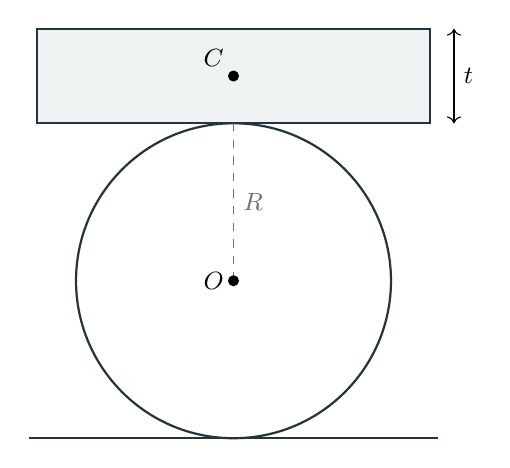
\begin{tikzpicture}
\draw[object](0,0)circle(2);\draw[object,fill=rulegray!35](-2.5,2)rectangle(2.5,3.2);
\draw[object](-2.6,-2)--(2.6,-2);
\draw[guide](0,0)--(0,2)node[midway,right]{$R$};
\draw[<->](2.8,2)--(2.8,3.2)node[midway,right]{$t$};
\fill(0,0)circle(2pt)node[left]{$O$};
\fill(0,2.6)circle(2pt)node[above left]{$C$};
\end{tikzpicture}
\figcaption{图5.10\quad 均匀板水平放在圆柱上，$C$在板截面中点，微小偏转遵守无滑动约束。}
\end{minipage}\end{center}

\workarea

\clearpage

\pdfbookmark[2]{第 11 题 菱形木条与圆盘的平衡}{q11}

\section*{第 11 题\quad 菱形木条与圆盘的平衡}

\tagline{M-05-11}

四根均匀木条的长度、质量分别相等，用光滑铰链连接成菱形，从顶点 $O$ 竖直悬挂。一均匀圆盘夹在下方两木条之间，接触光滑。每根木条长 $l=50\,\mathrm{cm}$、质量 $m=50\,\mathrm g$；圆盘半径 $r=8\,\mathrm{cm}$、质量 $M=200\,\mathrm g$。求图中木条与竖直线的夹角 $\theta$，并确定圆盘与木条的接触位置。

\begin{center}\begin{minipage}{\linewidth}\centering
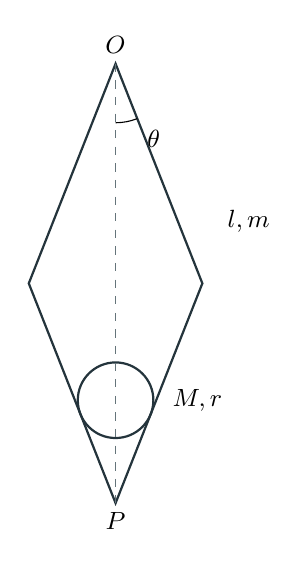
\begin{tikzpicture}
\coordinate(O)at(0,0);\coordinate(P)at(0,-5.580318676994);
\coordinate(U)at(1.102275313068,-2.790159338497);
\coordinate(V)at(-1.102275313068,-2.790159338497);
\coordinate(Cone)at(0,-2.790159338497);\coordinate(Ctwo)at(0,-4.273929989042);
\draw[object](O)--(U)--(P)--(V)--cycle;\draw[object](Ctwo)circle(.48);
\draw[guide](O)--(P);\node[above]at(O){$O$};\node[below]at(P){$P$};
\draw(0,-.75)arc(-90:-68.443095814:.75);\node[right]at(.28,-.95){$\theta$};
\node[right]at(.6,-4.273929989042){$M,r$};\node[right]at(1.3,-2){$l,m$};
\end{tikzpicture}
\figcaption{图5.11\quad 四边均长$l$，圆盘与下方两杆相切，角$\theta$相对竖直方向量起。}\end{minipage}\end{center}

\workarea

\clearpage

\pdfbookmark[2]{第 12 题 细绳张力与悬链线}{q12}

\section*{第 12 题\quad 细绳张力与悬链线}

\tagline{M-05-12}

质量分布均匀的柔软细绳长 $L$，线密度为 $\lambda$，静止悬于两个竖直支杆。两端向上的切线与竖直方向的夹角分别为 $\theta_1,\theta_2$，$0<\theta_1,\theta_2<\pi/2$。取左支杆为 $y$ 轴，水平向右为 $x$ 轴，左悬点为 $(0,H)$。
\begin{enumerate}\item 求两端张力。\item 推导悬链线方程，确定全部积分常量，并由所得方程求两端斜率和整段弧长。\end{enumerate}

\begin{center}\begin{minipage}{\linewidth}\centering
\begin{tikzpicture}
\draw[axis](0,-.2)--(0,3.9)node[above]{$y$};
\draw[axis](-.2,0)--(5.65,0)node[right]{$x$};\draw[object](5,0)--(5,3.3);
\draw[traj,domain=0:5,samples=110]plot(\x,{.5+2.2*(cosh((\x-2.2)/2.2)-1)});
\coordinate(A)at(0,1.694777396594);\coordinate(B)at(5,2.535708393558);
\fill(A)circle(1.7pt);\fill(B)circle(1.7pt);\node[left]at(A){$(0,H)$};
\draw[guide](A)--(-.65,2.458658172462);
\draw[guide](B)--(5.6,3.522861535308);
\draw(0,2.201777396594)arc(90:130.395062579:.507);
\node at(-.43,2.47){$\theta_1$};
\draw(5,3.042708393558)arc(90:58.708413156:.507);
\node at(5.27,3.3){$\theta_2$};
\node at(2.5,.15){全长$L$，线密度$\lambda$};
\end{tikzpicture}
\figcaption{图5.12\quad 两端均向上悬挂，$\theta_1,\theta_2$分别在端点切线与竖直线之间量取。}\end{minipage}\end{center}

\workarea

\end{document}
